\label{chapt:intro}

This is the introduction, why we are doing this analysis

\section{Background} % (fold)

\Company does this as per Figure~\ref{fig:companypic} seen below.

%% REFERENCE:
%%[htbp] (here, top, bottom, page).  ! means no restriction for placement
%%http://tex.stackexchange.com/questions/2275/keeping-tables-figures-close-to-where-they-are-mentioned help
\begin{figure}[H]
    \centering
    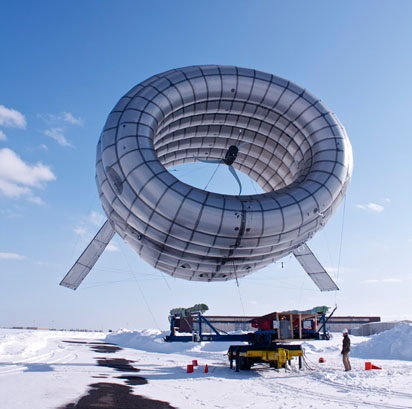
\includegraphics[width=0.6\textwidth]{companypic}
    \caption{Overview of the buoyant airborne technology \citep{companypicweb}}
    \label{fig:companypic}
\end{figure}


\section{Purpose}
The purpose of this report is to do this.
\begin{itemize}
    \item Do analysis on drum
    \item Development numerical algorithm for solving
\end{itemize}


\section{Scope} % (fold)

The scope of the report will be as follows.
